\documentclass{deimj}
%\usepackage[dvipdfm]{graphicx}
%\usepackage{latexsym}
%\usepackage{txfonts}
%\usepackage[fleqn]{amsmath}
%\usepackage[psamsfonts]{amssymb}
%\usepackage[deluxe]{otf}

\usepackage{graphicx}
\usepackage {subfig}

% 印刷位置調整 %
% 必要に応じて値を変更してください.
\hoffset -10mm % <-- 左に 10mm 移動
\voffset -10mm % <-- 上に 10mm 移動

\newcommand{\AmSLaTeX}{%
 $\mathcal A$\lower.4ex\hbox{$\!\mathcal M\!$}$\mathcal S$-\LaTeX}
\newcommand{\PS}{{\scshape Post\-Script}}
\def\BibTeX{{\rmfamily B\kern-.05em{\scshape i\kern-.025em b}\kern-.08em
 T\kern-.1667em\lower.7ex\hbox{E}\kern-.125em X}}

%\papernumber{DEIM Forum 2018 XX-Y}

\jtitle{非負値行列因子分解および回帰型ニューラルネットワークによる\\音響信号の可視化と信号予測}
%\jsubtitle{サブタイトル} <- サブタイトルを付けたいときはこの行の先頭の % を取る
\authorlist{%
 \authorentry{輪島 幸治}{Koji Wajima}{LA}% 
% \authorentry{古川 利博$^{\dagger}$}{Toshihiro Furukawa}{GTSU}% 
% \authorentry{佐藤 哲司$^{\dagger\dagger}$}{Tetsuji Satoh}{GTSU}% 
}

\affiliate[LA]{ロジカル・アーツ株式会社}{wajimak@nict.go.jp}

\begin{document}
\pagestyle{empty}

\maketitle
\section{はじめに}
情報社会の発展に伴う情報機器の普及で,
オンラインミーティングを始めとしたコミュニケーションが増加している.
%
オンラインミーティングにおける議事録作成では,
音声から自動でテキストデータを書き起こす
Amazon Transcribe\footnote{Amazon Transcribe:https://aws.amazon.com/jp/transcribe/}などのWebサービスも用いられてきている.

ビジネスだけでなく,コンシューマによるオンラインの配信活動も盛んになったことから,
音を対象としたメディアは重要インフラの電話やラジオ放送と同様に,
研究でも着目されるようになった.
%
一方で,音は,雑音を始めとした多くのノイズ信号によって,
単語や内容が認識できないなどの問題が発生して,
オンラインの業務環境に影響が発生する場合もある.
%
本研究では,オンラインコミュニケーションで特に重要とされている
音に着目して,音響信号の可視化および予測を試みた.
%
本研究で分析した音響信号を図\ref{figOriginal_Signal_Plot}に,
ノイズ信号を図\ref{fig:Noise_Signal_Plot}に示す.
図\ref{fig:Noise_Signal_Plot}のノイズ信号は,NHK Radio Englishの
音響信号にノイズ信号を合成して可視化した.

\vspace{-12pt}
\begin{figure}[htb]
  \begin{center}
    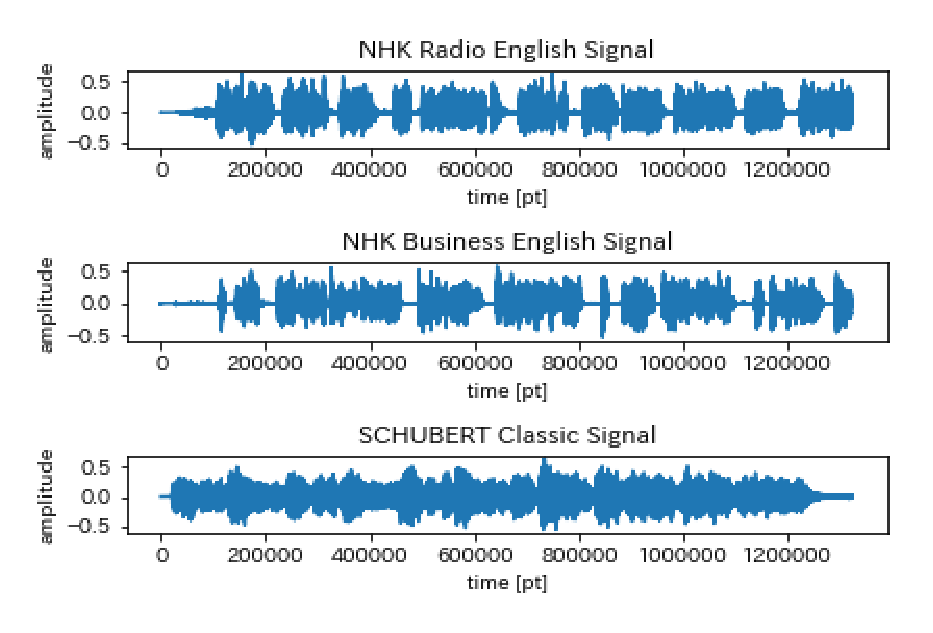
\includegraphics[width=0.78\columnwidth]{./eps/SoundFile_Original_Signal_Plot.eps}
\vspace{-6pt}
    \caption{分析対象の3種類の音響信号}
    \vspace{-4pt}
    \label{figOriginal_Signal_Plot}
    \vspace{-4pt}
  \end{center}
\end{figure}
%
\vspace{-15pt}
%
\begin{figure}[htb]
  \begin{center}
    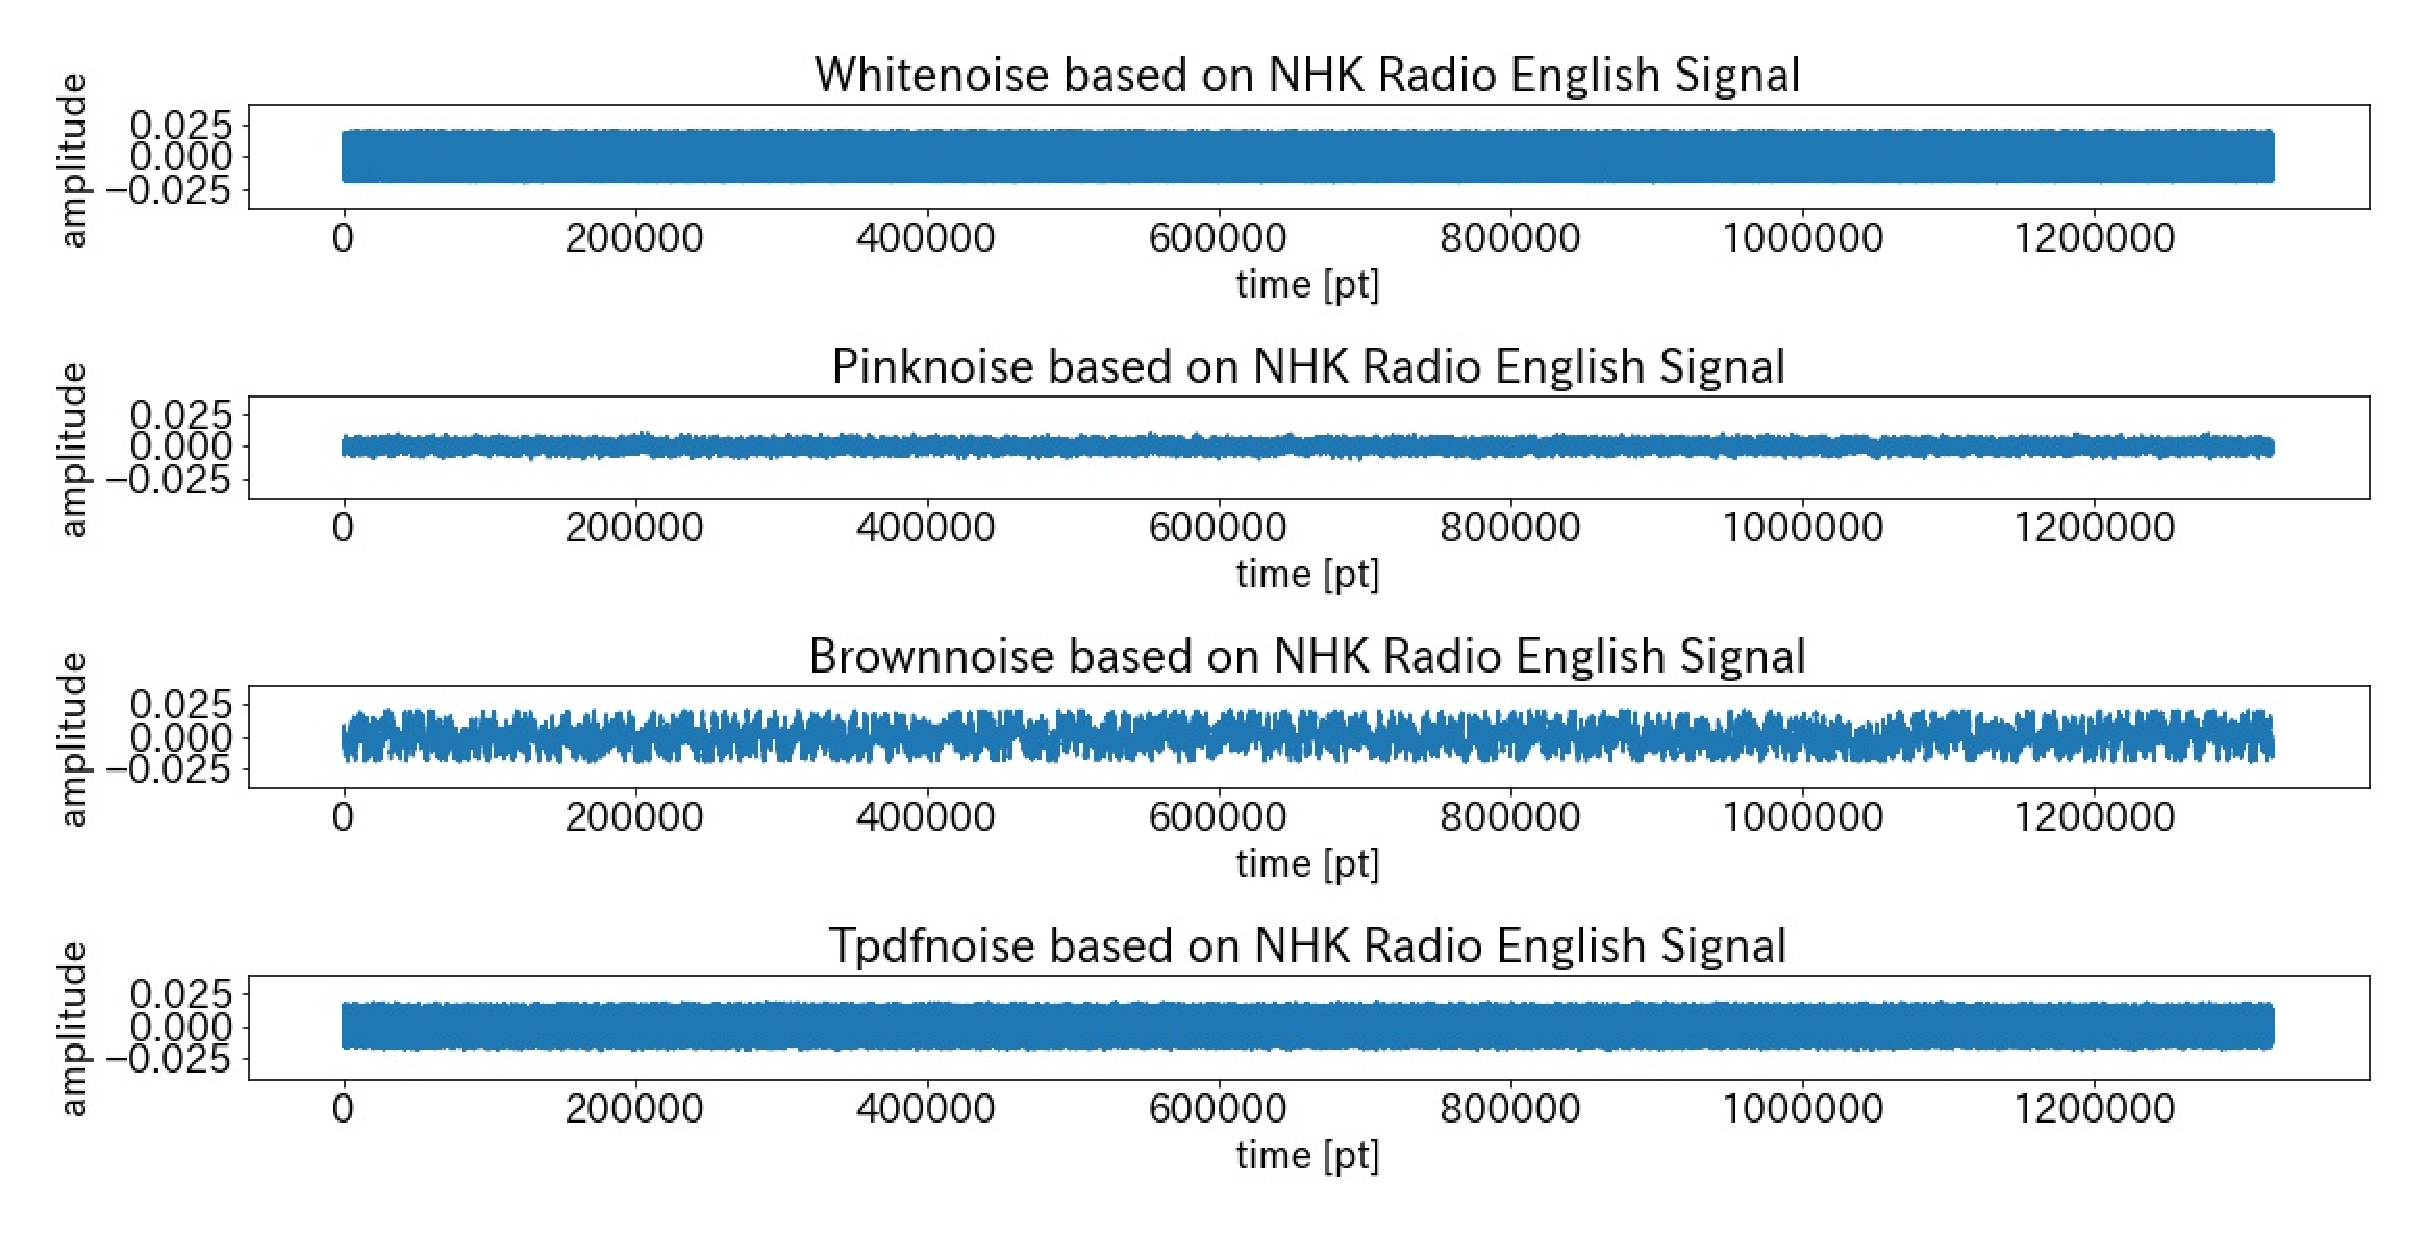
\includegraphics[width=0.78\columnwidth]{./eps/SoundFile_Noise_Signal_Plot.eps}
\vspace{-6pt}
    \caption{分析対象の4種類のノイズ信号}
    \label{fig:Noise_Signal_Plot}
  \end{center}
\end{figure}
\vspace{-12pt}

\renewcommand{\thefootnote}{\fnsymbol{footnote}}
\footnote[0]{
{\bf \scriptsize Visualization of acoustic signals and signal prediction using Nonnegative Matrix Factorization and Recurrent Neural Network}}
\footnotetext[0]{Koji Wajima$^{\dagger}$(wajimak@nict.go.jp, kwajima@ce.slis.tsukuba.ac.jp) \\ \scriptsize $^{\dagger}$Logical Arts Corporation, Osaka 541--0054, Japan, wajima@logical.co.jp}
\renewcommand{\thefootnote}{\arabic{footnote}}

%\newpage
さて,音を対象とした研究は,スピーカーなどのハードウェアやプログラムなど盛んに研究が行われている.
また,特許や実用新案が検索できるJ-PlatPat\footnote{特許情報プラットフォーム J-PlatPat:https://www.j-platpat.inpit.go.jp/}では,音源検索,言語識別,シーン抽出など放送分野を中心に出願され権利化多くの特許が確認できる.特許や実用新案だけでなく,音については,2015年から商標が,音楽的要素からなる音商標を登録の対象とした.

ここで,音声信号処理を始めとした信号処理では,雑音を始めとしたノイズ信号の影響で,
コミュニケーション内容が相手に十分に伝わらないことも少なくない.
%
図\ref{fig:Noise_Signal_Plot}のノイズ信号を
ヒストグラムにて可視化でした例を図\ref{fig:NoiseHistgram}に示す.

\vspace{-10pt}
\begin{figure}[h]
\begin{center}
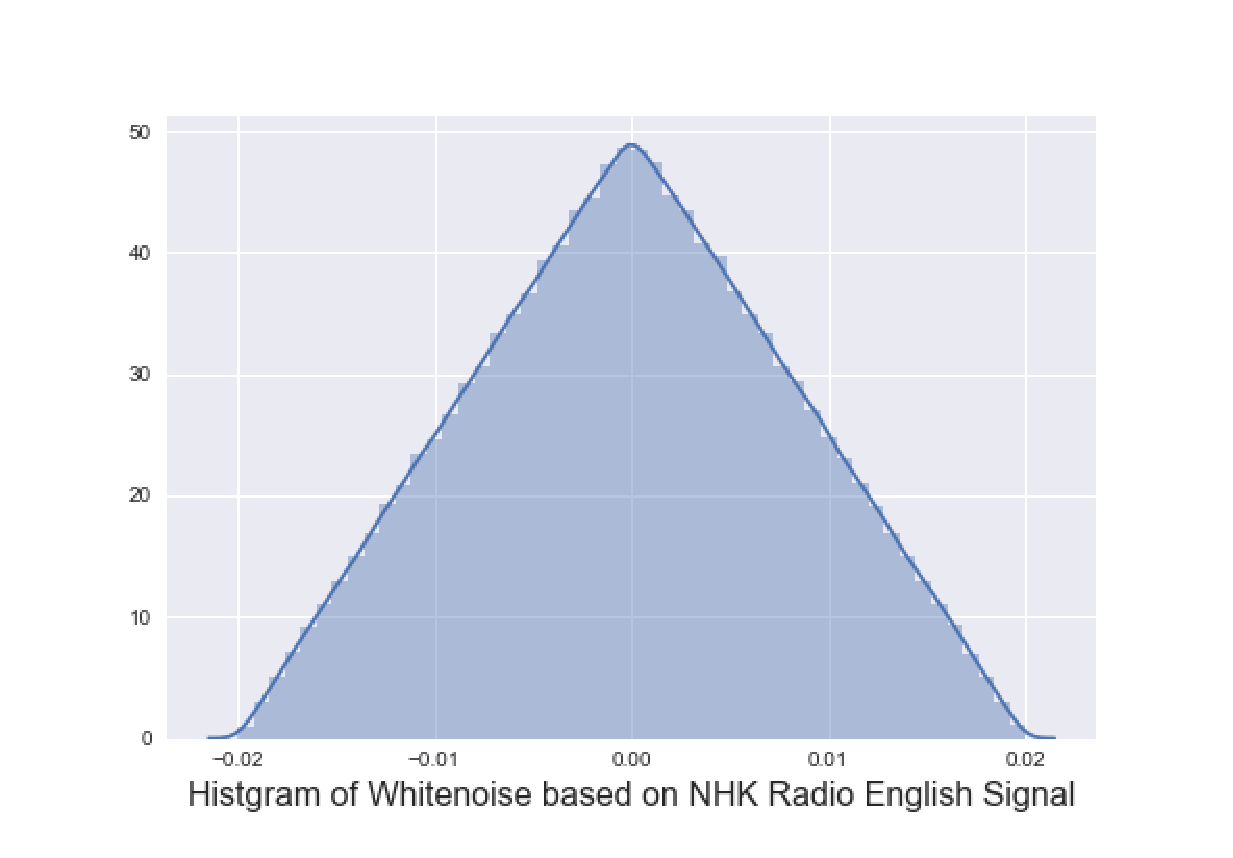
\includegraphics[width=0.4\columnwidth]{./eps/Signal_Plot/Signal_Whitenoise_Histgram.eps}%
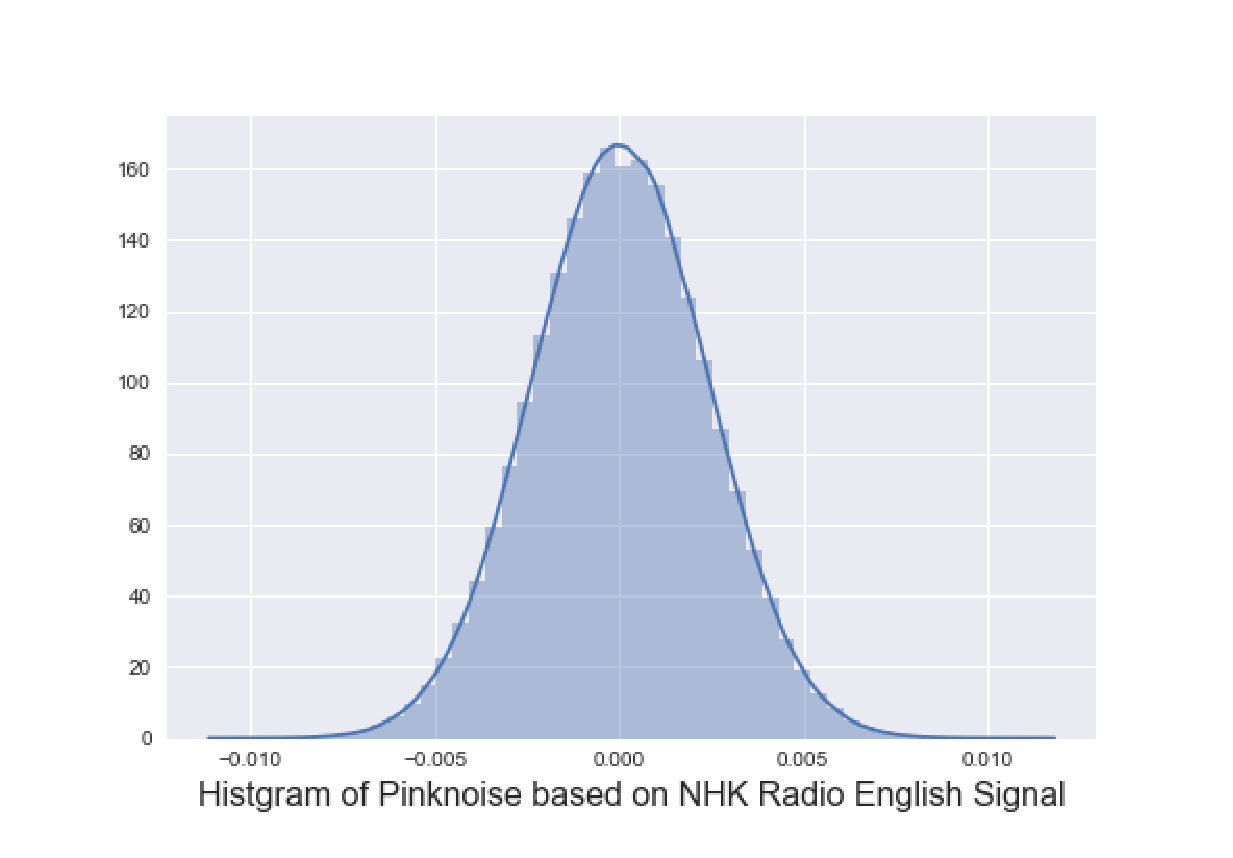
\includegraphics[width=0.4\columnwidth]{./eps/Signal_Plot/Signal_Pinknoise_Histgram.eps}\\
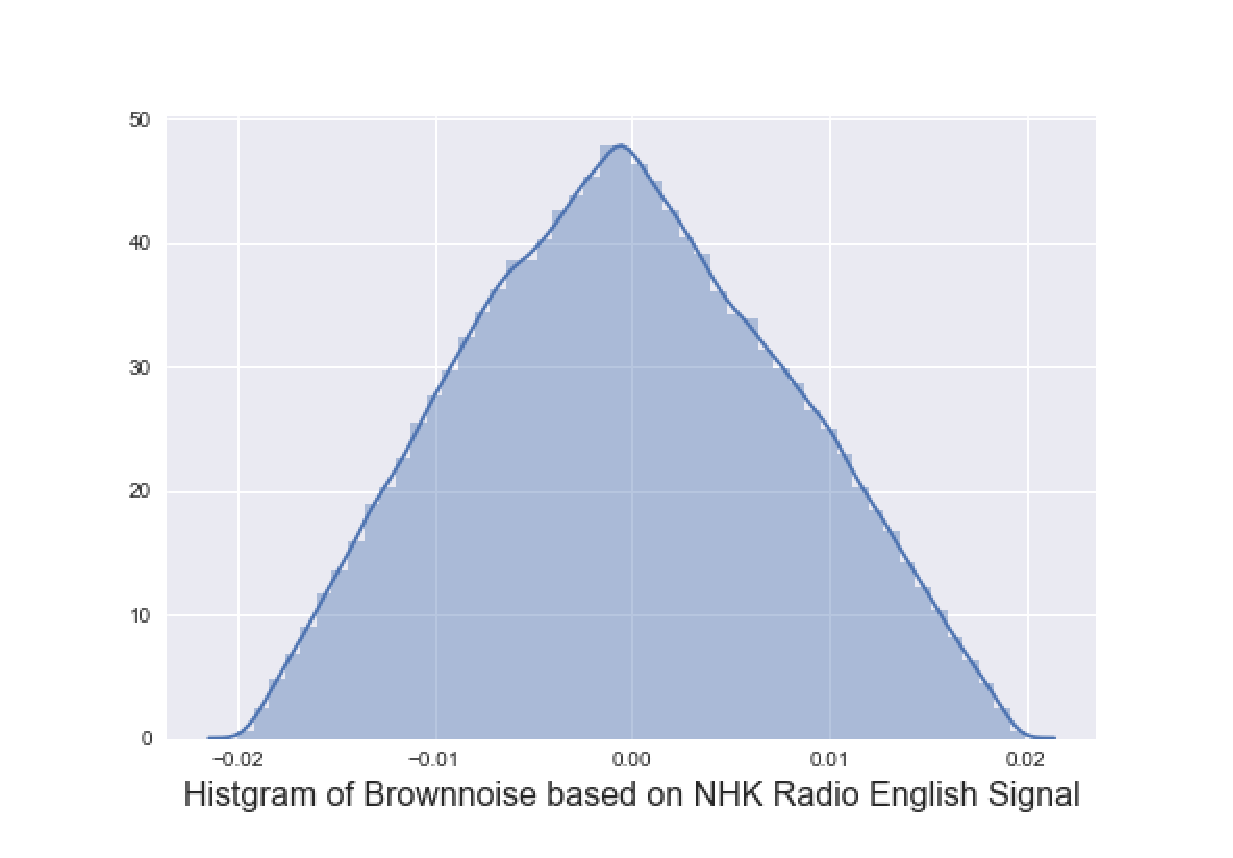
\includegraphics[width=0.4\columnwidth]{./eps/Signal_Plot/Signal_Brownnoise_Histgram.eps}%
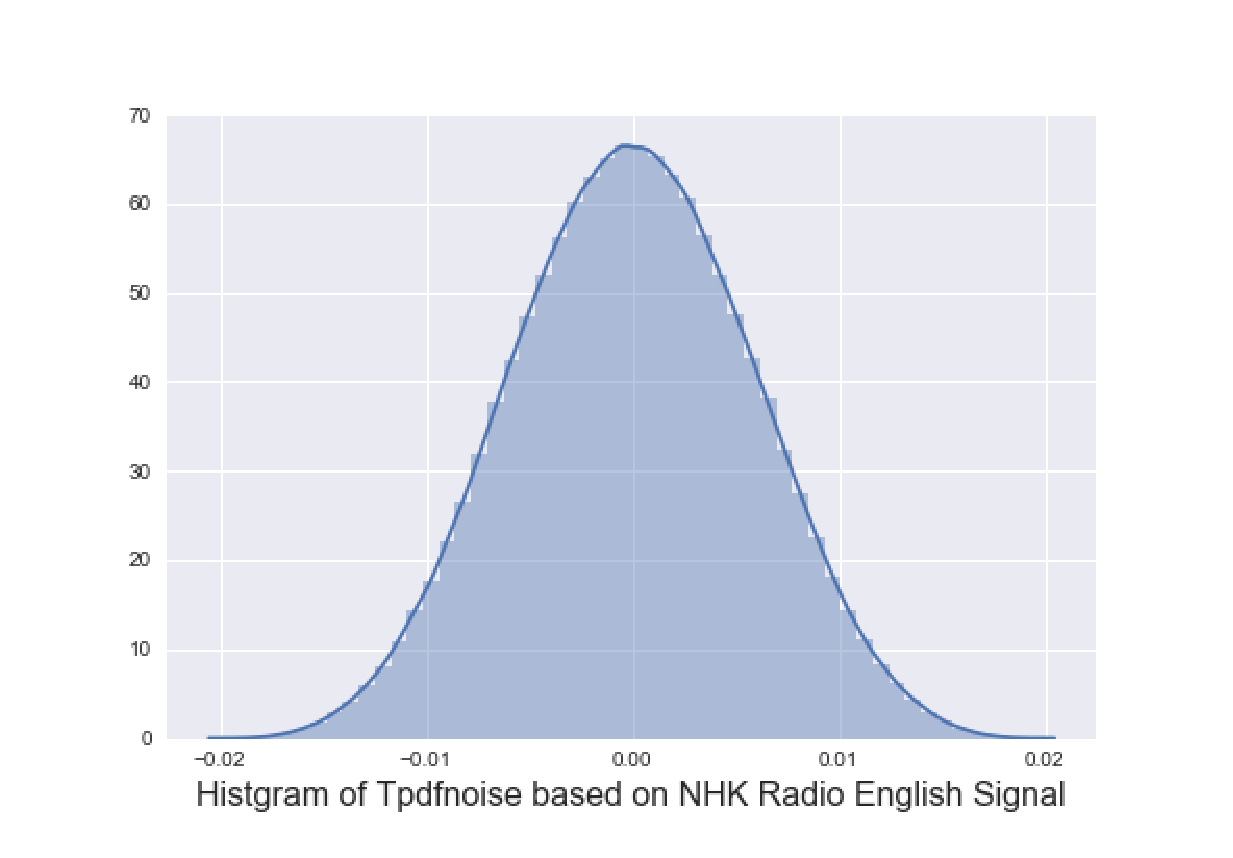
\includegraphics[width=0.4\columnwidth]{./eps/Signal_Plot/Signal_Tpdfnoise_Histgram.eps}%
\end{center}
%\vspace{-6pt}
\caption{Noise based on NHK Radio English Signal}
%\vspace{-6pt}
\label{fig:NoiseHistgram}
\end{figure}
\vspace{-15pt}

本研究では,ホワイトノイズ,ピンクノイズ,ブラウニアンノイズ,
三角形確率密度関数ノイズという4種類のノイズ信号を分析対象とした.
図\ref{fig:Noise_Signal_Plot}および図\ref{fig:NoiseHistgram}から明らかなように,
ノイズ信号はノイズ種類に応じて波形が異なる.
このため,ノイズ除去には多くの方法が必要とされている.

本研究では,音響信号など信号処理の分野で有効な非負値行列因子分解(NMF:Nonnegative Matrix Factorization)\cite{NMF}による可視化に用いる.また,回帰型ニューラルネットワーク(RNN:Recurrent Neural Network)を用いた信号予測で信号を予測できるかの評価を行った.
%https://www.jstage.jst.go.jp/article/jjsai/31/2/31_202/_pdf/-char/ja
%の予測における影響を明らかにすることを目的とした
%英文で名詞で使用する場合は[RNNs:Recurrent Neural Networks]

\vspace{-6pt}
\section{評価実験}
\vspace{-6pt}
本研究の実装は,NMFの実装に
scikit-learn\footnote{scikit-learn : https://scikit-learn.org/stable/},
回帰型ニューラルネットワークの実装には,Keras\footnote{Keras : https://keras.io/}を用いた\cite{chollet2015keras}.
%
また,音声データから数値行列への変換にはSoundFile
\footnote{SoundFile : https://pysoundfile.readthedocs.io/},ノイズ信号の生成および信号の合成については,SoX
\footnote{SoX:Sound eXchange : http://sox.sourceforge.net/}を用いている.

\newpage
\subsection{非負値行列因子分解を用いた可視化}
NMFを用いて音響信号を観測行列$Y$として,基底行列$H$と観測行列$Y$に行列分解を行い,
ホワイトノイズが含まれる音響信号を可視化した結果を図\ref{fig:NMF_Frobenius}および図\ref{fig:NMF_KL}に示す.
図\ref{fig:NMF_Frobenius}および図\ref{fig:NMF_KL}は時系列グラフであり,
縦軸は各基底,横軸が時間である.また,色が明るいほど係数が大きい.
%
図\ref{fig:NMF_Frobenius}と図\ref{fig:NMF_KL}の違いは,行列分解を行う際の乖離規準である.
図\ref{fig:NMF_Frobenius}では最小二乗法,図\ref{fig:NMF_KL}ではKullback Leiblerダイバージェンス規準を用いている.

\vspace{-10pt}
\begin{figure}[h]
  \begin{center}
\includegraphics[width=0.85\columnwidth]{./eps/NMF_HeatMap/HeatMap_Classic_whitenoise_longtime.eps}
%    \vspace{-10pt}
    \caption{Whitenoise - SCHUBERT Classic - 最小二乗法}
%    \vspace{-6pt}
    \label{fig:NMF_Frobenius}
  \end{center}
\end{figure}
%
\vspace{-20pt}
%
\begin{figure}[h]
  \begin{center}
\includegraphics[width=0.85\columnwidth]{./eps/NMF_HeatMap/HeatMap_Classic_whitenoise_longtime_kullbackleibler.eps}
%    \vspace{-10pt}
    \caption{Whitenoise - SCHUBERT Classic - Kullback Leibler }
%    \vspace{-6pt}
    \label{fig:NMF_KL}
  \end{center}
\end{figure}
\vspace{-15pt}

結果から,図\ref{fig:NMF_KL}と比較して,図\ref{fig:NMF_Frobenius}では明確な結果得られた.
また,本研究では,係数の大きい重要な基底を明らかにする場合における有効な乖離度規準は,
最小二乗法が適していることが明らかとなった.
%
このため,雑音の混合信号においても,
NMFを用いて乖離度規準や基底数を最適化することで,
音響信号の可視化できることが明らかとなった.
NMFが適用できれば不要な基底の除去と信号の再構成で,
ノイズ信号を除去することが期待できる.

\subsection{回帰型ニューラルネットワークを用いた信号の予測}
次に,RNNを用いてブラウンノイズとの混合信号の予測およびピンクノイズとの
混合信号の予測を図\ref{fig:NoiseBrownnoise}および図\ref{fig:PinknoiseNoise}に示す.
%
図\ref{fig:NoiseBrownnoise}および図\ref{fig:PinknoiseNoise}は,左側が混合信号の波形である.
右側が前半部分の青色で着目されているのが混合信号の波形で,
後半部分の赤色で着目されているのが混合信号を元にRNNで信号を予測した波形である.

結果から,RNNの適用は,ブラウンノイズ混合信号の予測においては,
図\ref{fig:NoiseBrownnoise}から,RNNによって目的の値に近い値を予測できた.
%
一方で,ピンクノイズ混合信号を予測した図\ref{fig:PinknoiseNoise}では,傾向としては類似の波形だが,
ブラウンノイズ混合信号の予測と比較して,不明瞭な予測結果となった.
このことから,RNNによる予測で,ブラウンノイズよりもピンクノイズが影響が大きいという結果が得られた.

\vspace{-6pt}
\section{まとめ}
\vspace{-6pt}
本稿では,音響信号の可視化および信号予測を目的に,
NMFとRNNを用いて,ノイズを混合した信号の分析を試みた.
結果,NMFでは,有効な乖離度規準することにより音響信号の可視化が行えた.
%
また,RNNでは,予測に影響のあるノイズ信号が明らかとなり,
ブラウンノイズのようにノイズ信号との混合信号でも期待された予測が得られる結果も得られた.

\newpage
\begin{figure}
%\begin{figure}
\vspace{-6pt}
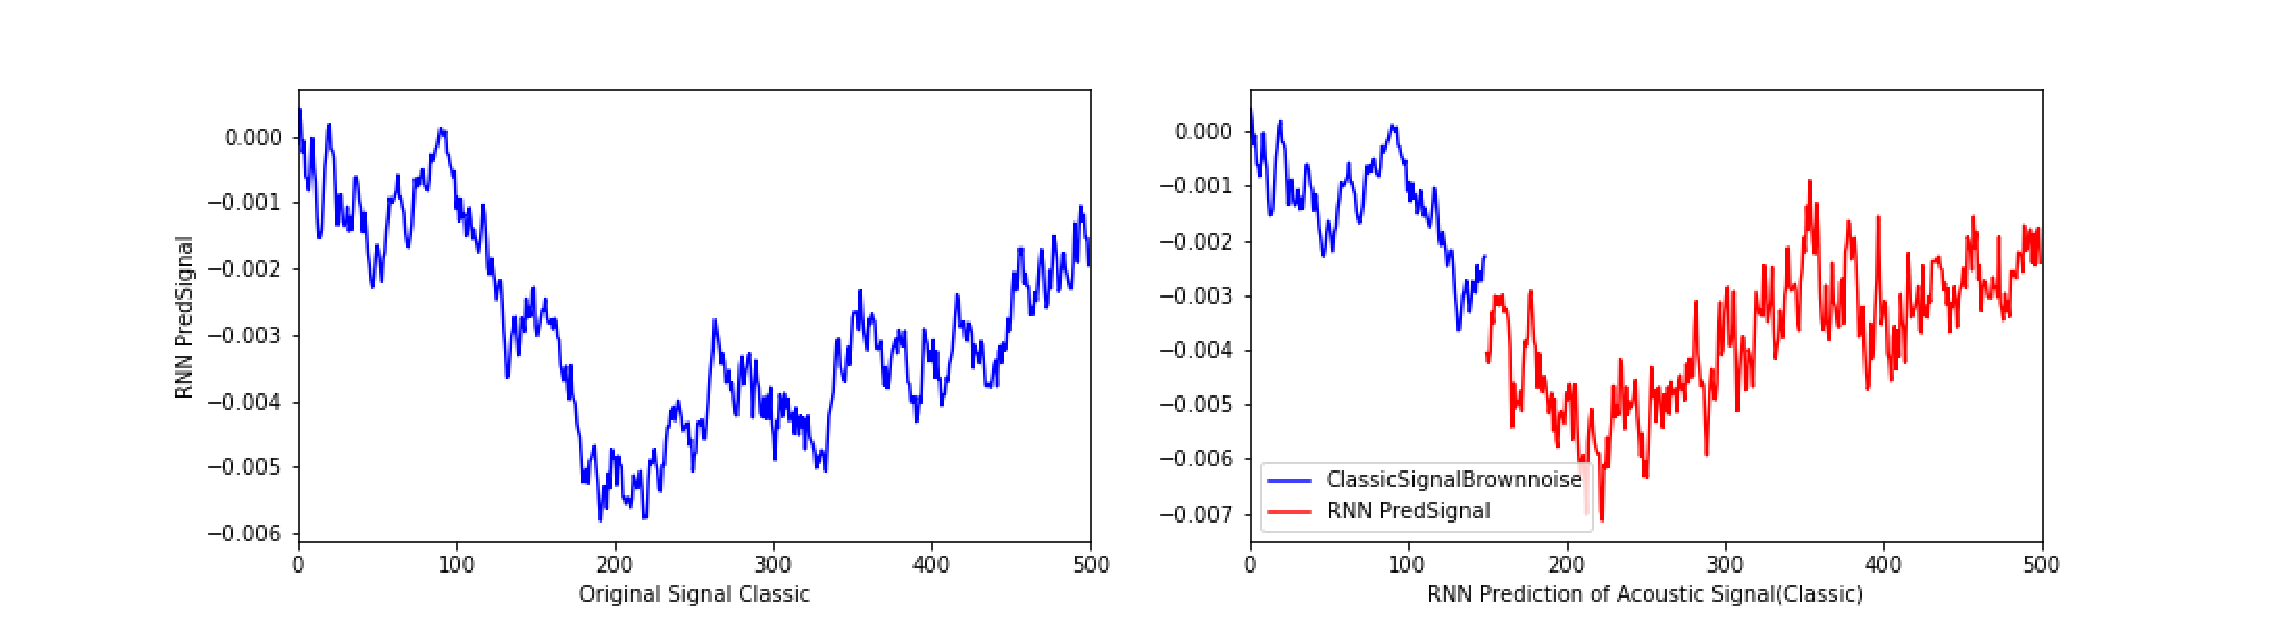
\includegraphics[width=0.85\columnwidth]{./eps/RNN_Brownnoise/RNN_Brownnoise_Classic.eps}\\
\label{fig:Noise}
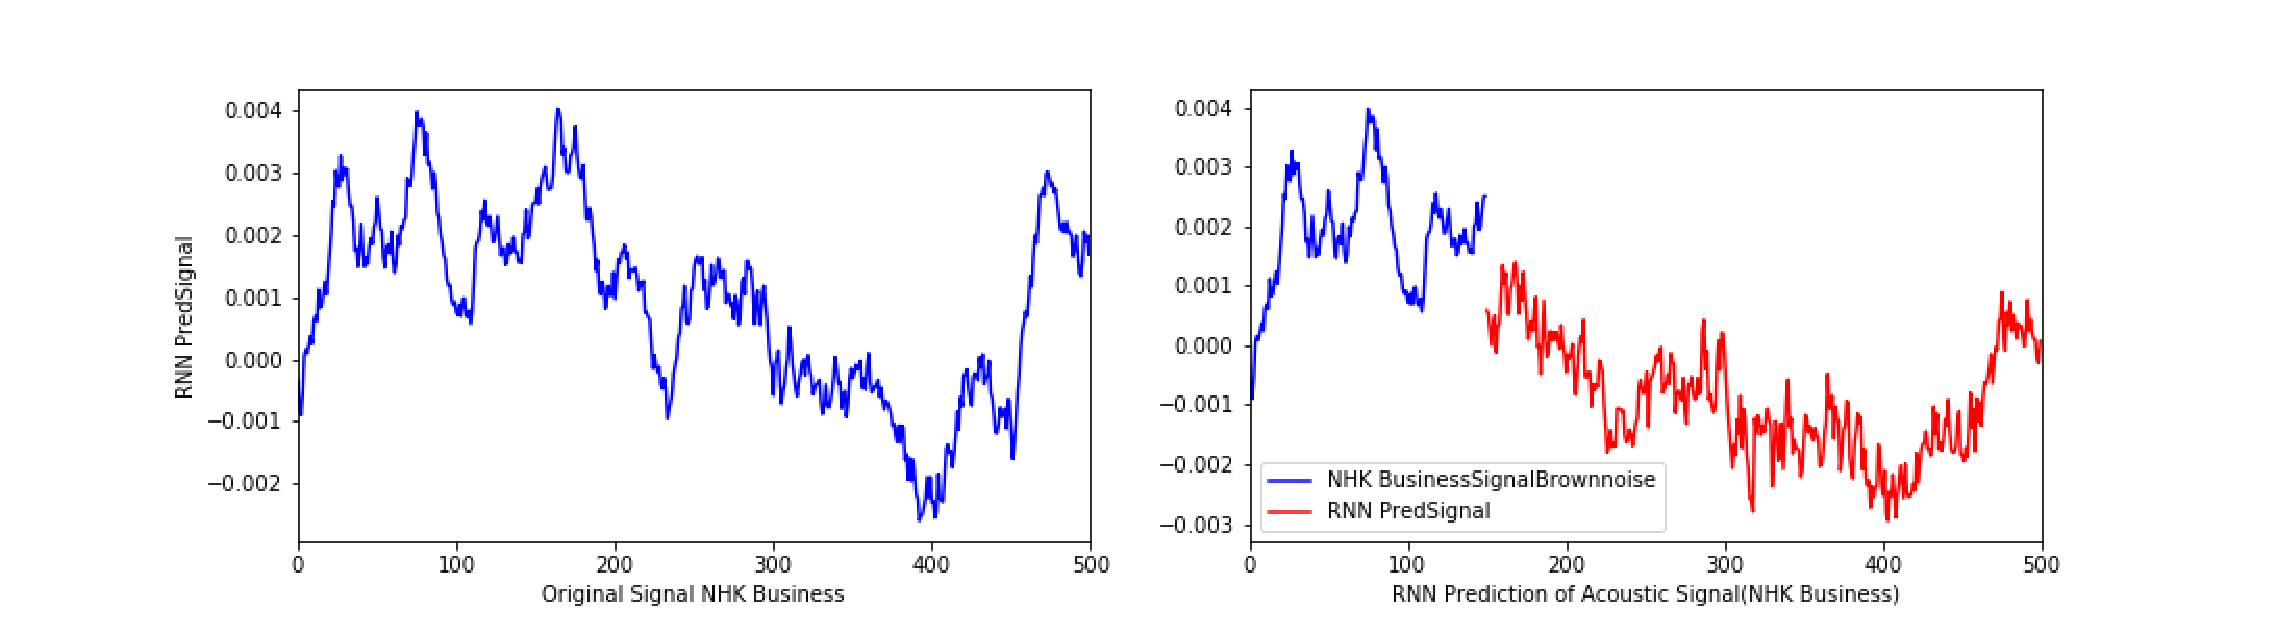
\includegraphics[width=0.85\columnwidth]{./eps/RNN_Brownnoise/RNN_Brownnoise_NHKBusiness.eps}\\
\label{fig:Noise}
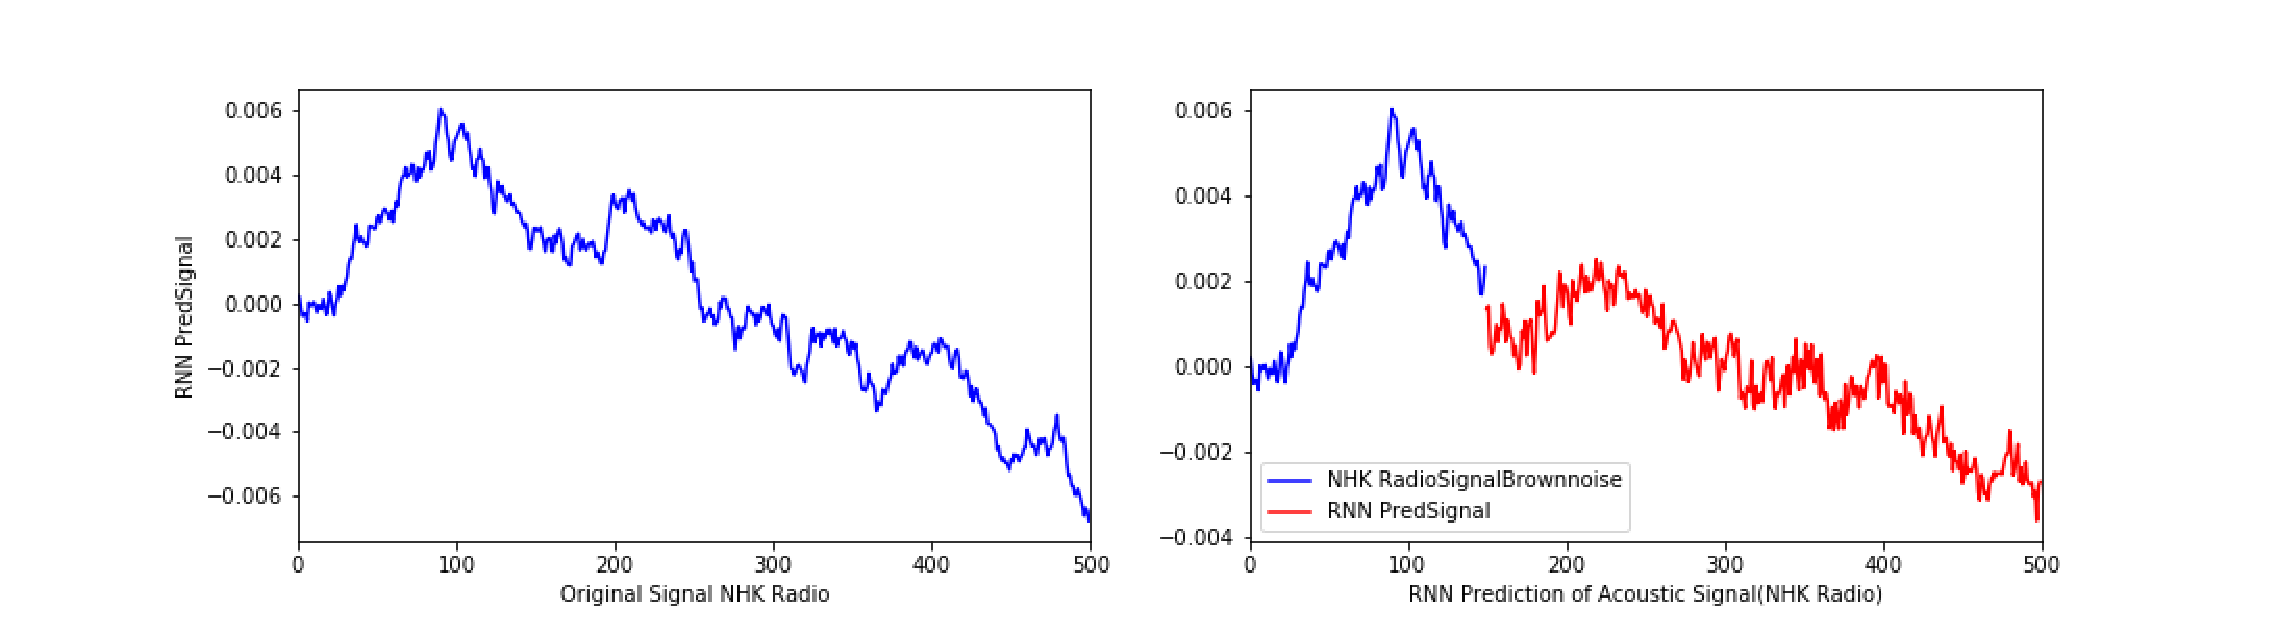
\includegraphics[width=0.85\columnwidth]{./eps/RNN_Brownnoise/RNN_Brownnoise_NHKRadio.eps}
\vspace{-3pt}
\caption{ブラウンノイズ混合信号のRNNによる予測}
\vspace{-6pt}
\label{fig:NoiseBrownnoise}
\vspace{-6pt}
\end{figure}
%
\vspace{-10pt}
%
\begin{figure}
%\begin{figure}
\vspace{-6pt}
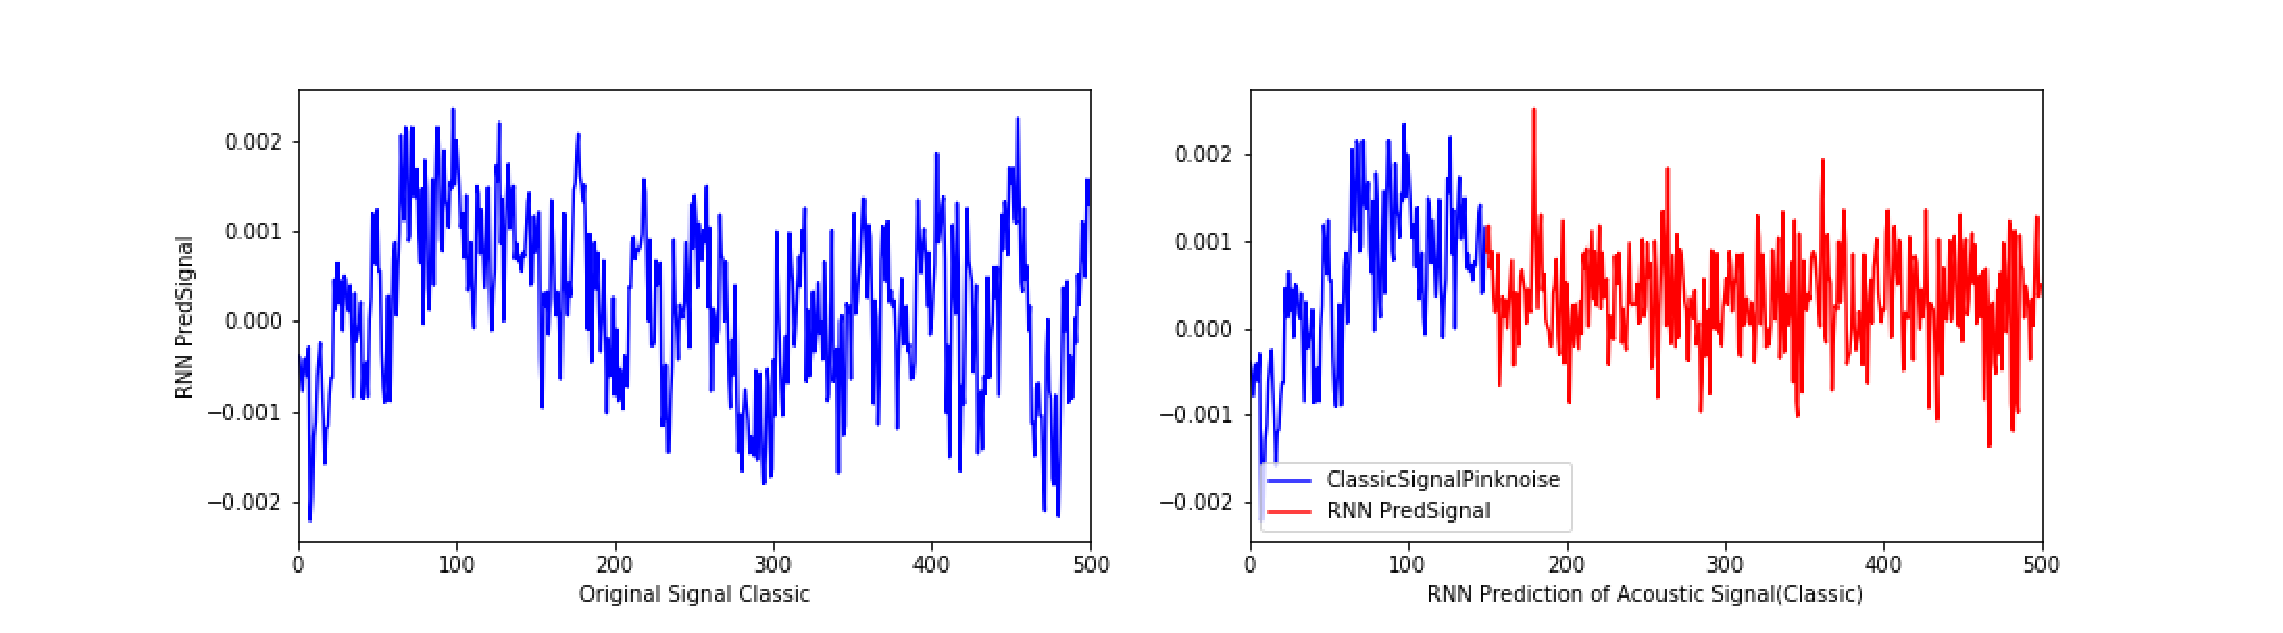
\includegraphics[width=0.85\columnwidth]{./eps/RNN_Pinknoise/RNN_Pinknoise_Classic.eps}\\
\label{fig:Noise}
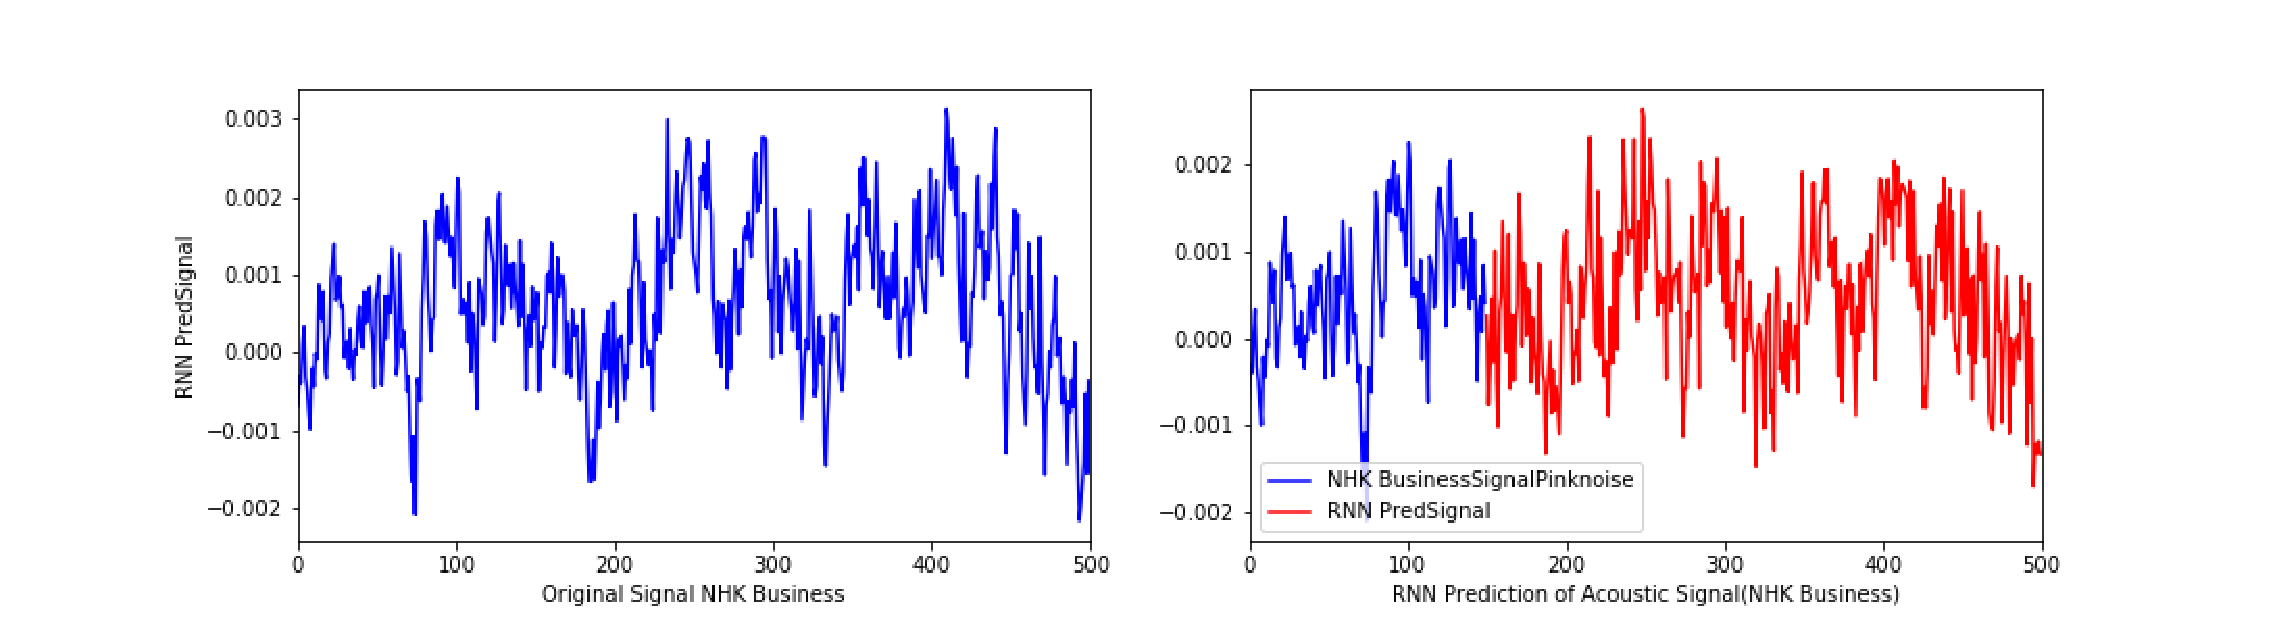
\includegraphics[width=0.85\columnwidth]{./eps/RNN_Pinknoise/RNN_Pinknoise_NHKBusiness.eps}\\
\label{fig:Noise}
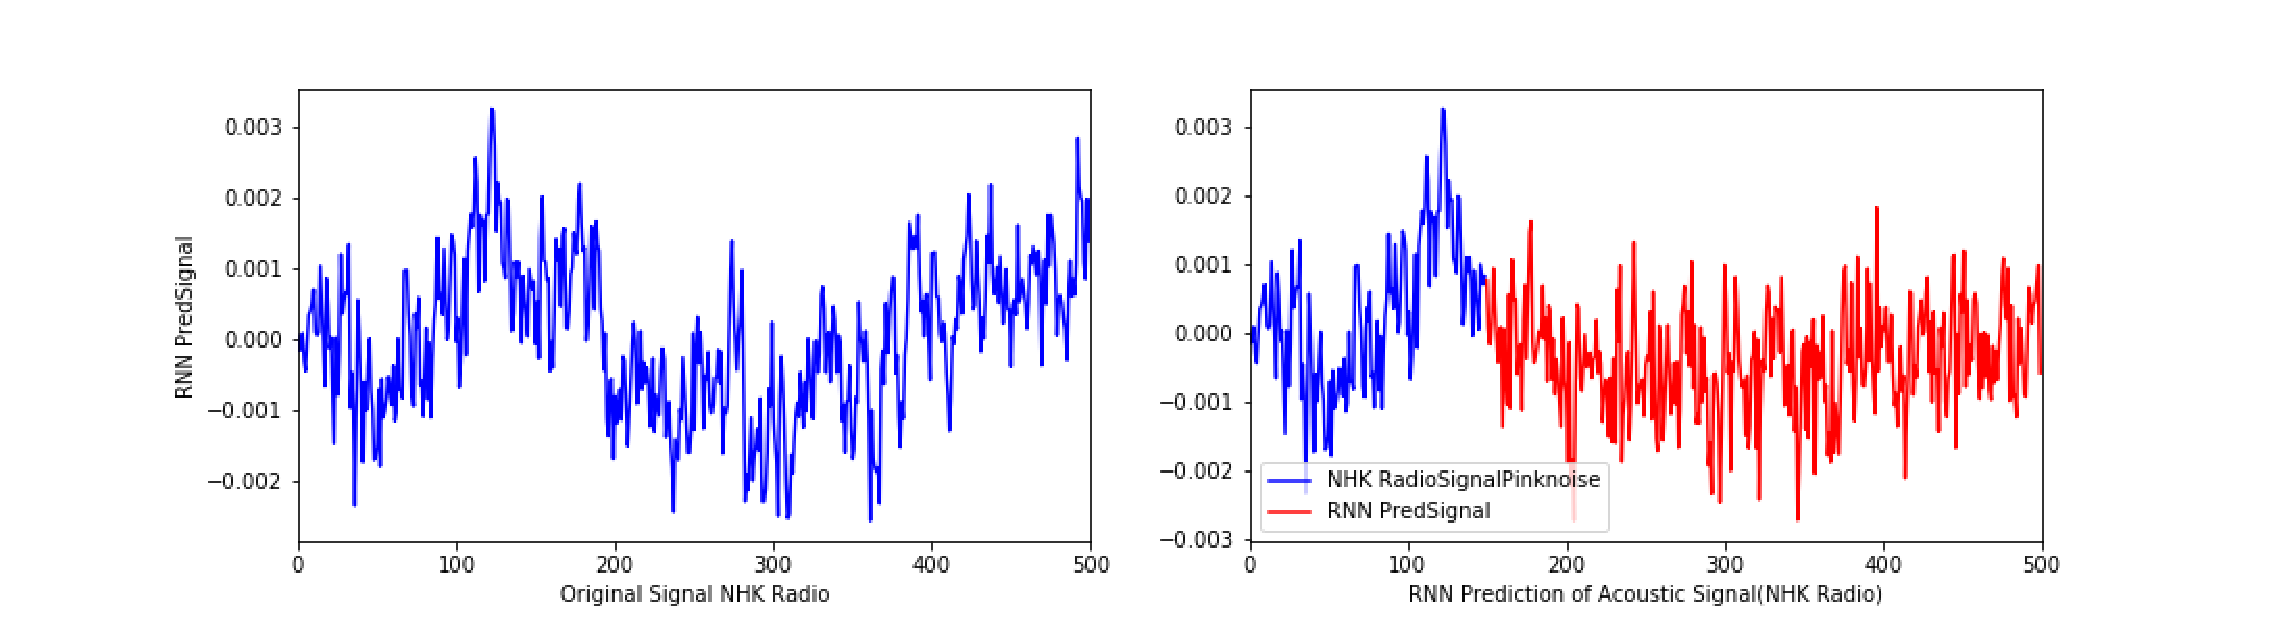
\includegraphics[width=0.85\columnwidth]{./eps/RNN_Pinknoise/RNN_Pinknoise_NHKRadio.eps}
\vspace{-3pt}
\caption{ピンクノイズ混合信号のRNNによる予測}
\vspace{-10pt}
\label{fig:PinknoiseNoise}
\vspace{-10pt}
\end{figure}

また,本稿では,テレワークの広がりから音響信号を対象としたが,
デジタル世代と呼ばれる世代はツール,メディア,コミュニティが
アナログ世代と異なり多くの課題が指摘されている\cite{book_dentsu}.
今後の研究課題としては,コミュニティにおける表現,
アナログとデジタルとの比較,研究成果を働き方改革などのビジネスに適用するなど,
多くの課題解決のために,NMFやRNNなど時系列データに効果的な分析手法を検討していきたい.

%7
\vspace{-8pt}
\section*{謝辞}
\vspace{-8pt}
本稿の研究成果だが,実際に音声信号を体験して,研究の着想を頂いた.
ここに記して,国立研究開発法人 情報通信研究機構の皆様に謝辞を示します.
%
合わせて,2021年4月30日に博士(情報学)の学位を授与頂いた筑波大学,
筑波大学の博士後期課程における連携大学院の株式会社電通の木暮 啓教授\footnote{ビジネス・クリエーション・センター 電通総研 シンクタンク・グループ},株式会社電通の皆様,博士後期課程時に在籍していた株式会社セールスフォース・ジャパン(投稿時点:株式会社セールスフォース・ドットコム)の皆様,エンバーポイント株式会社の皆様(所属時:エクスペリアンジャパン株式会社),
横河ソリューションサービス株式会社の皆様に謝辞を示します.
%https://www.jstage.jst.go.jp/article/jasj/68/11/68_KJ00008328910/_article/-char/ja

%\vspace{30mm} <- 文献が本文と近すぎるときは適宜利用してください.
%\vspace{2em}
\bibliographystyle{junsrt}
\bibliography{ipsj_bibliography}




\end{document}
